% Generated by scripts/txt2tex.py from chapters/chapter_04.txt. Edit the TXT, not this file.
\chapterquestion{איך נולדת תשובה שלמה, אם המכונה כותבת אותה חתיכה אחר חתיכה ואינה יודעת מראש איך היא תסתיים?}
\chapter{כיצד מודל שפה מייצר תשובה}\label{ch:04}
\section{הסצנה בהילוך איטי}
חזרו אל המטבח של הקוראת. השאלה "למה הבצק שלי לא תופח, ומה אפשר לעשות עכשיו?" כבר נשלחה, ובתוך המכונה היא הפכה, כפי שראינו בפרק הקודם, לזרם של מספרים. עכשיו מתחילה התשובה לזרום: מילה מופיעה על המסך, ועוד אחת, ועוד אחת, בקצב שמזכיר מישהו שמקליד בצד השני של הקו.
נאט את הסצנה עד כמעט עצירה. דמיינו שהתשובה נפתחת, למשל, במילים "יש כמה סיבות אפשריות", משפט שהספר בחר לשם ההדגמה. בשבריר השנייה שבין "יש" לבין "כמה" המערכת לא שלפה משפט מוכן ממגירה. היא עשתה דבר צנוע יותר, ומפתיע יותר: ניחשה מה בא עכשיו.
כולנו עושים זאת בשיחה. חבר אומר "נתראה מחר ב...", ועוד לפני שסיים צצות בראש כמה השלמות, חלקן סבירות יותר מאחרות. מודל שפה (language model) הפך את ההרגל הזה לשיטה. בניסוח המתמטי, ההסתברות של טקסט שלם מתפרקת לשרשרת של שאלות קטנות, וכל אחת מהן שואלת: מה הסיכוי ליחידה הבאה, בהינתן כל מה שכבר נכתב \cite{S-ch04-03,S-ch04-04}. כך נוצר הטקסט, מתחילתו לסופו, יחידה אחר יחידה \cite{S-ch04-03}. נעקוב אחרי המילה "כמה" מרגע שהשאלה התקבלה ועד שהופיעה על המסך.
\section{לקבל את הטקסט, ולפרק אותו}
השלב הראשון נשמע מובן מאליו: לקבל את הטקסט כמו שהוא. אבל זו החלטה. מחברי הדוח על GPT-2 (2019) מתארים עיבוד מקדים שמקובל במודלי שפה, כמו המרת כל האותיות לאותיות קטנות, שמגביל את המחרוזות שהמודל מסוגל לייצג. את GPT-2 הם תכננו כך שיוותר על עיבוד שמאבד מידע, ויוכל להעניק הסתברות לכל מחרוזת Unicode \cite{S-ch04-04}.
עכשיו צריך לפרק את הטקסט ליחידות. למה לא פשוט למילים? כי אוצר מילים שלם הוא עצום, וכל מילה שלא הופיעה בו הופכת לסימן כללי של "לא ידוע". ואם נפרק לאותיות בודדות, הרצפים מתארכים מאוד, ואות אחת נושאת הרבה פחות משמעות ממילה שלמה \cite{S-ch04-06}. שפה היא בעיה פתוחה, שבה תמיד צצות מילים חדשות, בעוד שאוצר המילים של מודלי תרגום נוירוניים הוגבל בדרך כלל, נכון ל-2016, ל-30,000 עד 50,000 מילים \cite{S-ch04-02}.
הפתרון הוא דרך ביניים: חלקי מילים (subword units). מילה נפוצה נשארת יחידה אחת, ומילה נדירה מתפרקת לחלקים \cite{S-ch04-06}. סנריך ועמיתיו התאימו ב-2016 לפירוק כזה את שיטת קידוד זוגות הבתים (Byte Pair Encoding, BPE): מתחילים מתווים בודדים, מוצאים את זוג הסמלים הסמוכים השכיח ביותר, ממזגים אותו לסמל חדש, וחוזרים חלילה. מספר המיזוגים הוא ההגדרה היחידה שצריך לבחור \cite{S-ch04-02}. בדוגמה מהמאמר, המילה lower, שלא הופיעה במילון שממנו נלמדו המיזוגים, פורקה ל-low ול-er \cite{S-ch04-02}.
ב-GPT-2 הרעיון הזה מופעל על בתים במקום על אותיות, ולכן האוסף הבסיסי שלו מונה רק 256 סמלים \cite{S-ch04-04}. אוצר המילים המלא שלו מונה 50,257 טוקנים: 256 בתים, 50,000 מיזוגים וטוקן מיוחד אחד שמסמן סוף טקסט \cite{S-ch04-06}.
ומה קורה למילה "תופח" מהשאלה של הקוראת? ייתכן שהיא תישאר שלמה, וייתכן שתתפרק, נניח, ל"תופ" ול"ח". זה פירוק להמחשה בלבד: הספר לא בדק טוקנייזר מסוים על עברית, והפירוק בפועל תלוי באוצר המילים של כל מערכת.
\begin{conceptbox}{טוקן (token)}
טוקן הוא יחידת הטקסט הבסיסית שמודל שפה קורא וכותב. הוא יכול להיות מילה שלמה, חלק ממילה, תו או בית, לפי אוצר המילים של הטוקנייזר \cite{S-ch04-06}. אוצר המילים הוא רשימה סגורה: ב-GPT הראשון היו בה 40,478 טוקנים, וב-GPT-2 50,257 \cite{S-ch04-06}. לכל טוקן ברשימה יש מספר סידורי.
פרט שקל לפספס: המודל סופר טוקנים, לא מילים. חלון ההקשר של GPT-2, כלומר כמות הטקסט שהוא מסוגל להביא בחשבון בבת אחת, מוגדר ב-1,024 טוקנים \cite{S-ch04-04}.
\end{conceptbox}
\section{כתובת במרחב של משמעויות}
מספר סידורי ברשימה עדיין אינו משמעות. ב-2013 תיארו מיקולוב ועמיתיו את המצב שהיה נפוץ אז: מערכות רבות התייחסו למילים כאל יחידות אטומיות, אינדקסים באוצר מילים בלי שום מושג של דמיון ביניהם \cite{S-ch04-05}. מבחינתן, "בצק" רחוקה מ"עיסה" בדיוק כמו מ"מטרייה".
החלופה היא לייצג כל מילה כווקטור, כלומר כרשימה ארוכה של מספרים, כך שמילים דומות נוטות להיות קרובות זו לזו במרחב, ויכולות להיות ביניהן כמה דרגות של דמיון \cite{S-ch04-05}. מיקולוב ועמיתיו הציעו דרך יעילה ללמוד וקטורים כאלה מאוסף עצום של טקסט \cite{S-ch04-05}. המאמר מביא מעבודה קודמת דוגמה שנעשתה מפורסמת: אם לוקחים את הווקטור של King, מחסירים ממנו את הווקטור של Man ומוסיפים את זה של Woman, הווקטור הקרוב ביותר לתוצאה הוא זה של Queen \cite{S-ch04-05}. משמעות הופכת לגאומטריה.
לייצוג כזה קוראים שיבוץ (embedding). ב-Transformer, הארכיטקטורה שעליה נשענים מודלי השפה בפרק הזה, כל טוקן מקבל וקטור נלמד, שבמאמר המקורי משנת 2017 אורכו 512 מספרים \cite{S-ch04-01}. הווקטורים האלה נלמדים יחד עם המודל כולו \cite{S-ch04-01}, ומיד אחר כך עוברים שלב שמערב בהם מידע מהמילים שמסביב.
\section{להקשיב למילים הנכונות}
בשאלה של הקוראת, "עכשיו" נקשרת ל"לעשות", ו"שלי" נקשרת ל"בצק". כדי להבין מילה צריך לדעת למי מהשכנות שלה להקשיב. על זה בדיוק מופקד מנגנון הקשב (attention).
המאמר "Attention Is All You Need" (2017) הציג ארכיטקטורה שמוותרת על רקורסיה (recurrence), כלומר על מעבר על הקלט מילה אחר מילה בתוך הרשת, ונשענת כולה על קשב \cite{S-ch04-01}. כל מיקום ברצף שולח מעין שאילתה (query). כל מיקום, כולל השולח עצמו, מציע מפתח (key), שמתאר במה הוא יכול לעזור, וערך (value), שהוא התוכן שהוא מוסר. הפלט הוא סכום משוקלל של הערכים: ככל שהשאילתה מתאימה יותר למפתח, כך המשקל של הערך גבוה יותר \cite{S-ch04-01}. במאמר פועלים במקביל שמונה "ראשי" קשב, וכל אחד מהם יכול להתמקד בקשר אחר \cite{S-ch04-01}.
עוד כלל אחד חשוב לסצנה שלנו: בזמן הכתיבה, כל מיקום רשאי לפנות רק אל מה שלפניו \cite{S-ch04-01}. המודל לא מציץ במילים שעוד לא נכתבו, ממש כמו שאי אפשר לשמוע את סוף המשפט של החבר לפני שאמר אותו.
\section{ציון לכל טוקן, הסתברות לכל המשך}
בסוף העיבוד, טרנספורמציה לינארית נלמדת מעניקה ציון לכל אחד מהטוקנים באוצר המילים, ופונקציה בשם softmax הופכת את הציונים להסתברויות לטוקן הבא \cite{S-ch04-01}. הולצמן ועמיתיו קוראים לציונים האלה logits \cite{S-ch04-03}.
בחזרה לרגע שאחרי "יש". דמיינו שההסתברויות נראות כך: "כמה" 0.46, "מספר" 0.22, "סיבות" 0.12, "לא" 0.05, וכל שאר אוצר המילים חולק את היתר. מספרים להמחשה בלבד.
ההתפלגות הזאת לא תמיד נראית אותו דבר. הולצמן ועמיתיו מראים שלפעמים היא שטוחה, עם המון המשכים סבירים, כמו אחרי פתיחה של ציטוט, ולפעמים מחודדת: אחרי "I ate the pizza while it was still" כמעט כל ההסתברות מרוכזת במילה אחת, "hot" \cite{S-ch04-03}.
\section{הרגע שבו נבחרת מילה}
הסתברויות אינן החלטה. את ההחלטה מקבלת אסטרטגיית פענוח (decoding strategy), כלל שקובע איך בוחרים את הטוקן הבא \cite{S-ch04-07}, והכלל הזה לבדו יכול לשנות מאוד את איכות הטקסט שמפיק אותו מודל \cite{S-ch04-03}.
הדרך הפשוטה היא בחירה חמדנית (greedy): בכל שלב לוקחים את הטוקן הסביר ביותר. בספריית Transformers של Hugging Face זו ברירת המחדל, והיא מתאימה לפלטים קצרים, אבל בטקסט ארוך היא מתחילה לחזור על עצמה \cite{S-ch04-07}. חיפוש אלומה (beam search) עוקב אחרי כמה רצפים במקביל ובוחר את זה שההסתברות הכוללת שלו הגבוהה ביותר \cite{S-ch04-07}. אלא שלפי הולצמן ועמיתיו, ניסיון למקסם הסתברות מוביל לטקסט תפל, לא קוהרנטי, או כזה שנתקע בלולאות של חזרות \cite{S-ch04-03}.
החלופה היא דגימה (sampling): הגרלה לפי ההתפלגות, שבה לכל טוקן שההסתברות שלו אינה אפס יש סיכוי להיבחר, ולכן פחות חזרות ויותר גיוון \cite{S-ch04-07}. אבל דגימה טהורה עלולה להפיק גיבוב, כפי שהולצמן ועמיתיו הדגימו על GPT-2 \cite{S-ch04-03}. דרכי הביניים מצמצמות את ההגרלה: ב-top-k מגרילים רק מתוך k הטוקנים הסבירים ביותר, וב-top-p, שנקראת גם דגימת גרעין (nucleus), מגרילים מתוך הקבוצה הקטנה ביותר שההסתברויות שלה מצטברות לפחות ל-p. גודל הקבוצה משתנה בכל הגרלה לפי צורת ההתפלגות \cite{S-ch04-03}.
הגדרה נוספת היא הטמפרטורה (temperature): מחלקים את הציונים במספר t לפני ה-softmax. ערך קטן מ-1 מטה את ההתפלגות לטובת הטוקנים הסבירים, והורדת הטמפרטורה משפרת את האיכות במחיר של פחות גיוון \cite{S-ch04-03}. כאן "טמפרטורה" היא פרמטר כוונון של הדגימה. בפרק 6 נפגוש את אותה מילה במשמעות אחרת, ואסור לבלבל ביניהן.
\begin{figure}[htbp]
\centering
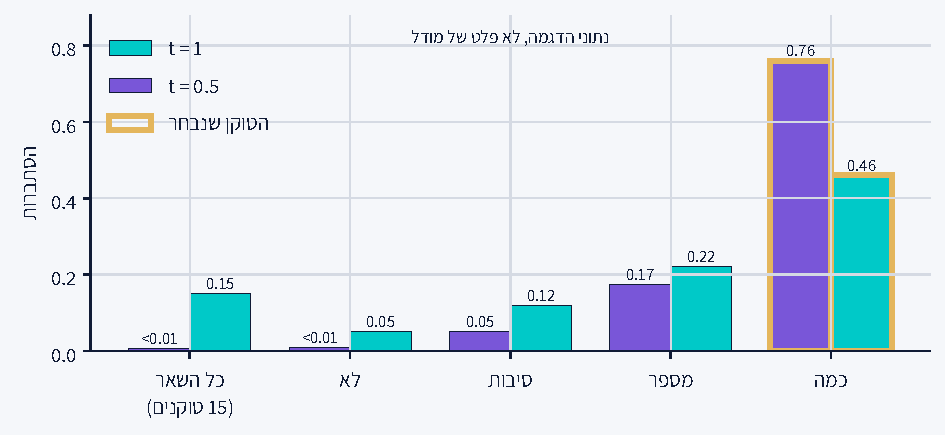
\includegraphics[width=\linewidth]{assets/charts/fig4_1_temperature.pdf}
\caption{אותם ציונים, שתי טמפרטורות}\label{fig:4.1}
\figurenote{נתוני הדגמה, לא פלט של מודל · מקור: נתוני הדגמה (ציונים מומצאים); הנוסחה מ-\cite{S-ch04-03}}
\end{figure}
\begin{behindbox}{הלולאה, טוקן אחר טוקן}
המפענח ב-Transformer הוא אוטו-רגרסיבי: הוא מייצר סמל אחד בכל פעם, וכל סמל שכבר נוצר נכנס כקלט ליצירת הסמל הבא \cite{S-ch04-01}. בתיעוד של Hugging Face הלולאה נראית בקוד כמעט כפי שהיא: מחשבים ציונים, בוחרים את הגבוה שבהם, מצרפים את הטוקן שנבחר לקלט וחוזרים על הכול \cite{S-ch04-07}.
בסצנה שלנו: "יש" נבחרה ונוספה לסוף הרצף. כל הרצף, השאלה ו"יש", עובר שוב את הדרך, ורק אז מופיעה "כמה". כך הלאה, עד סוף התשובה. גם GPT-3 מתואר על ידי מפתחיו כמודל שפה אוטו-רגרסיבי \cite{S-ch04-08}.
\end{behindbox}
\section{תשעה צעדים, ותרשים שמודה בפשטותו}
\begin{figure}[htbp]
\centering
% Figure 4.2: from the question to the answer in nine steps (9 block nodes + generation loop).
% Read right to left, snaking down; block 8 ("בחירת טוקן") is highlighted in Gold.
\begin{bookdiagram}[x=1cm,y=1cm]
  \tikzset{st/.style={blk,text width=3.6cm,minimum height=12mm}}
  \node[st] (s1) at (12.2,0)    {שאלת משתמש};
  \node[st] (s2) at (7.1,0)     {קבלת הטקסט};
  \node[st] (s3) at (2.0,0)     {פירוק לטוקנים};
  \node[st] (s4) at (2.0,-2.3)  {ייצוג מספרי};
  \node[st] (s5) at (7.1,-2.3)  {עיבוד קשב};
  \node[st] (s6) at (12.2,-2.3) {חישוב ציוני טוקנים};
  \node[st] (s7) at (12.2,-4.6) {המרה להסתברויות};
  \node[st,draw=gold,line width=2.2pt] (s8) at (7.1,-4.6) {בחירת טוקן};
  \node[st] (s9) at (2.0,-4.6)  {הרכבת תשובה};
  \foreach \n in {1,...,9}{\node[num] at ($(s\n.north east)+(-0.08,-0.08)$) {\n};}
  \foreach \a/\b in {1/2,2/3,3/4,4/5,5/6,6/7,7/8,8/9}{\draw[flow] (s\a) -- (s\b);}
  \draw[loop,solid,line width=1.4pt] (s8.south) -- ++(0,-0.8) -| ($(s4.west)+(-0.7,0)$) -- (s4.west);
  \node[font=\footnotesize\headingfont,text=violet] at (7.1,-5.75) {הטוקן שנבחר מצטרף לרצף, והלולאה חוזרת};
\end{bookdiagram}

\caption{מהשאלה אל התשובה, בתשעה צעדים}\label{fig:4.2}
\figurenote{תרשים הסברתי ומפושט, לא ארכיטקטורה מלאה · מקור: מסגרת הספר, על בסיס \cite{S-ch04-01}, \cite{S-ch04-03}, \cite{S-ch04-04} ו-\cite{S-ch04-07}}
\end{figure}
התרשים הזה מוותר על פרטים רבים כדי שאפשר יהיה לראות משהו: הוא הסבר מפושט, ולא תיאור מלא של ארכיטקטורת מודל. ב-Transformer המקורי מתווסף לכל וקטור, פעם אחת בכניסה, קידוד של מיקומו ברצף. שכבות הקשב, ולצידן שכבות עיבוד שאינן קשב, מוערמות שש פעמים זו על גבי זו \cite{S-ch04-01}. המודל המקורי נבנה לתרגום מכונה, משני חלקים, מקודד ומפענח \cite{S-ch04-01}, ו-GPT-2 מבוסס על הארכיטקטורה הזאת בשינויים \cite{S-ch04-04}.
גם קנה המידה נעלם מהתרשים: הגרסה הגדולה של GPT-2 כוללת 1.5 מיליארד פרמטרים \cite{S-ch04-04}, ו-GPT-3, שהוצג ב-2020, כולל 175 מיליארד \cite{S-ch04-08}. במה שמוצרים מסחריים מוסיפים סביב המודל הספר אינו עוסק. ולבסוף, הבלוקים נראים כמו תהליך שרץ פעם אחת, בעוד שבפועל רובם חוזרים לכל טוקן חדש. זה תפקידו של חץ הלולאה.
\begin{thinkbox}
אם הקוראת תשאל את אותה שאלה פעמיים, בדיוק באותן מילים, ותקבל שתי תשובות בניסוח שונה, איזו מהן היא "התשובה של המערכת"? ואם טמפרטורה נמוכה הופכת את התשובות לדומות יותר זו לזו, האם היא גם הופכת אותן לנכונות יותר? מה בדיוק הייתם רוצים למדוד כדי לדעת?
\end{thinkbox}
\section{התשובה שעל המסך}
כעבור כמה שניות מסתיימת התשובה. הקוראת רואה פסקה רהוטה, שלמה, כאילו נכתבה במחשבה תחילה. עכשיו אנחנו יודעים שהיא נבנתה ניחוש אחר ניחוש, וכל מילה בה נבחרה מתוך התפלגות. רהיטות היא תוצר של הסתברויות, לא הוכחה לאמת.
וכאן עולה השאלה הבאה, זו שהקוראת עצמה כבר מתחילה לשאול: איך יודעים אם תשובה כזאת טובה? על כך בפרק הבא.
\begin{insightsbox}
\begin{itemize}
\item מודל שפה אינו שולף תשובות מוכנות. הוא מנחש בכל צעד את הקטע הבא של הטקסט, על סמך כל מה שנכתב עד אז \cite{S-ch04-03,S-ch04-04}.
\item הטוקן, ולא המילה, הוא יחידת העבודה. שיטות כמו BPE מאפשרות לייצג גם מילה שהמערכת מעולם לא ראתה, באמצעות חלקים מוכרים \cite{S-ch04-02,S-ch04-06}.
\item שיבוצים הופכים מספר סידורי למיקום במרחב, וקשב מאפשר לכל מיקום ברצף לשקלל מידע מהמיקומים האחרים \cite{S-ch04-01,S-ch04-05}.
\item אותן הסתברויות יכולות להוליד טקסטים שונים מאוד: הבחירה בין חמדנות, חיפוש אלומה, דגימה וטמפרטורה משנה את התוצאה \cite{S-ch04-03,S-ch04-07}.
\item כל תרשים של התהליך הוא פישוט. מה שחשוב לזכור ממנו הוא הלולאה: כל מילה שנבחרה הופכת לחלק מהקלט של המילה הבאה \cite{S-ch04-01}.
\end{itemize}
\end{insightsbox}
